\documentclass[11pt]{article}

\usepackage{amsmath,amssymb,amsthm,setspace,tabto,fancyhdr,sectsty,mathtools}
\usepackage{titleps}
\usepackage[left=1.00in,right=1.00in,top=0.75in,bottom=1.50in]{geometry}
\usepackage{graphicx}

% change this line
\graphicspath{ {assets/note5/} }

% start pdfinlimg (GPLv3, https://github.com/zerotoc/pdfinlimg/blob/master/pdfinlimg.sty)
\newcommand{\pdfinlimg}[5]{
\makebox[#1cm][l]{\immediate\pdfliteral{
  q
  #3 0 0 #4 0 0 cm
  #1 0 0 #2 0 0 cm
  0.885 0 0 0.885 0 0 cm 
  BI
  /W #3
  /H #4
  /CS /RGB
  /BPC 8
  /F [ /AHx /Fl ]
  ID
  #5>
  EI
  Q
}\vbox to #2cm{}}
}
% end pdfinlimg

% BEGIN PARAGRAPH STUFF
\usepackage[utf8]{inputenc}
\usepackage[english]{babel}
 
\setlength{\parindent}{4em}
% \setlength{\parskip}{1em}
\renewcommand{\baselinestretch}{1}
% END PARAGRAPH STUFF

% useful commands
\DeclarePairedDelimiter{\ceil}{\lceil}{\rceil}
\DeclarePairedDelimiter{\floor}{\lfloor}{\rfloor}

\newpagestyle{footers} {
    \sethead{}{}{}
    \setfoot{\small Intro to Crypto and Blockchain, Note \notenum}{\thepage}{\small Lin, Akhtar}
    \footskip = 45pt
}

\fancypagestyle{firstpage} {
    \vspace*{3\baselineskip}
    \footskip = 0pt
    \renewcommand{\headrulewidth}{6pt}
    \chead{\rule{\textwidth}{6pt} \vspace{20pt}\\}
    \lhead{\setstretch{1.05}\Large\fontfamily{lmdh}\selectfont
    Introduction to Cryptocurrencies and Blockchain 
    \\ Lin, Akhtar}
    \rhead{\huge \fontfamily{lmdh}\selectfont    Note \notenum}
    \lfoot{\small Intro to Crypto and Blockchain, Note \notenum}
    \rfoot{\small Lin, Akhtar}
}
    
\sectionfont{\Large\fontfamily{lmdh}\selectfont}

% for initial paragraph indent
\usepackage{indentfirst}

% UPDATE THIS FOR EVERY NEW NOTE
\newcommand{\notenum}{5}

\pagestyle{footers}

\begin{document}
    \thispagestyle{firstpage}
    \vspace*{2\baselineskip}
    \section*{Cryptocurrency Mining: Proof-of-Work Consensus}
    
    Bitcoin mining is the process through which new bitcoins enter the network and is also what keeps the network healthy and resistant to malicious parties---an arms race that rewards those who invest the most into their hardware. But why do miners mine? What incentives do they have, and most importantly, is it profitable? In this section, we will explain in depth the design and mechanics behind Bitcoin mining, taking into account various mining incentives.
    
    \section*{Recap: What a Miner Does}
    
    \noindent In a nutshell, a Bitcoin miner accomplishes the following six tasks:
    
    \begin{enumerate}
        \item \textit{Download} the entire Bitcoin blockchain to store the entire transaction history.
        \item \textit{Verify} incoming transactions by checking signatures and confirming the existence of valid bitcoins.
        \item \textit{Create} a block using collected valid transactions.
        \item \textit{Find} a valid nonce to create a valid block header (this is the ``mining'' part).
        \item \textit{Hope} that your block is accepted by other nodes and not defeated by a competitor block.
        \item \textit{Profit!} Coinbase transacation rewards miners for their work.
    \end{enumerate}
    
    The Bitcoin miner maintains the Bitcoin network's health by creating valid blocks and participating honestly in the Proof-of-Work protocol. They ensure that (hopefully) only valid blocks make their way into the blockchain, receiving a bitcoin reward in exchange (also functioning as a mechanism through which new coin created in the Bitcoin network).
    
    \section*{Block Difficulty --- Analogy}
    
    Imagine a game in which you are blindfolded, throwing darts randomly at a dart board. (Say for simplicity that all your darts are guaranteed to land on the dartboard.) There is an equal likelihood of hitting any given point on the dartboard. If one of your darts lands within a certain radius $d$ from the center, then you get a reward. Throwing faster allows for more hits per second, granting a higher likelihood of any of your darts land within the target distance and a higher chance of winning the reward. 
    
    Now imagine competing with many other blindfolded individuals to hit the target first. The difficulty of hitting the target is inversely proportional to $d$. In other words, it's harder to hit a smaller target and easier to hit a larger one. To control how many rewards are distributed within a given period of time, $d$ changes depending on the average time taken to hit the target. This way, if people get better at throwing darts, then $d$ gets smaller, and vice versa.
    
    \section*{Block Difficulty --- Puzzle Prerequisites}
    
    Instead of blindly throwing darts at a dartboard, mining in Bitcoin involves solving a hash puzzle that results in a valid block. Miners race each other to find a nonce that makes the following inequality true:
    $$H\big(nonce~||~H(previous~block~header)~||~merkle~root\big)~<~target$$
    
    Hash puzzles need to be computationally difficult. If finding the proof-of-work required little work, then reaching consensus would be difficult (See Note 4). This is why in the analogy, we blindfolded the dart-throwers. Hash puzzles also must have a variable cost, allowing for adjustments as the global hashrate increases. Finally, hash puzzles should be easily verifiable by all other nodes in the network. There should not be a need for a central authority to verify nonce validity. Every miner simply rehashes the nonce to verify validity. In the dart analogy, darts stick to the dartboard, so to verify, others simply have to take their blindfolds off to verify.
    
    \section*{Block Difficulty --- Adjustment}
    
    \noindent The following is the equation to adjust the difficulty of the hash puzzle used in Bitcoin:
    
    $$\mathit{difficulty}~=~\mathit{difficulty~*~two\_weeks~/~time\_to\_mine\_prev\_2016\_blocks}$$
    
    We use the ratio between two weeks and the time to mine 2016 blocks because the target block time is 10 minutes. 
    
    $$\mathit{2016~blocks~*~10~\frac{min}{block}=20160~min=2~weeks}$$
    
    If the time to mine 2016 blocks is greater than two weeks, then the hash puzzle is too hard. The ratio is less than 1, so the difficulty scales down. If the time to mine 2016 blocks is less than two weeks, then the hash puzzle is too easy. The ratio is greater than 1, so the difficulty scales up. The block difficulty is always inversely proportional to the time required to mine the previous 2016 blocks.
    
    \section*{How to Profit From Mining}
    
    For the Bitcoin miner, the following equations are true.
    \begin{align*}
        \begin{split}
            MINING\_REWARD~&=~BLOCK\_REWARD~+~TX\_FEES \\
            MINING\_COST~&=~HARDWARE\_COST~+~OPERATING\_COSTS
        \end{split}
    \end{align*}
    
    If mining rewards exceed mining costs, then a Bitcoin miner will profit. In the next sections, we will analyze each of the components in the above equations.
    
    \section*{Block Reward}
    
    A Bitcoin miner receives bitcoin for every confirmed block. Currently, the block reward is 12.5 BTC per block. The potential for profit (finding the proof-of-work first, broadcasting it, and getting it confirmed for block reward) provides incentive for honest behavior in the Bitcoin network. To receive the block reward, the miner must include a special transaction back to themselves, called the coinbase transaction. The block reward in the coinbase transaction is designed to half every 210,000 blocks. This is done to cap the total number of bitcoin that will ever be produced. There is a finite number of bitcoin, and by the year 2140, there will be 21,000,000 BTC (the supply cap.)
    
    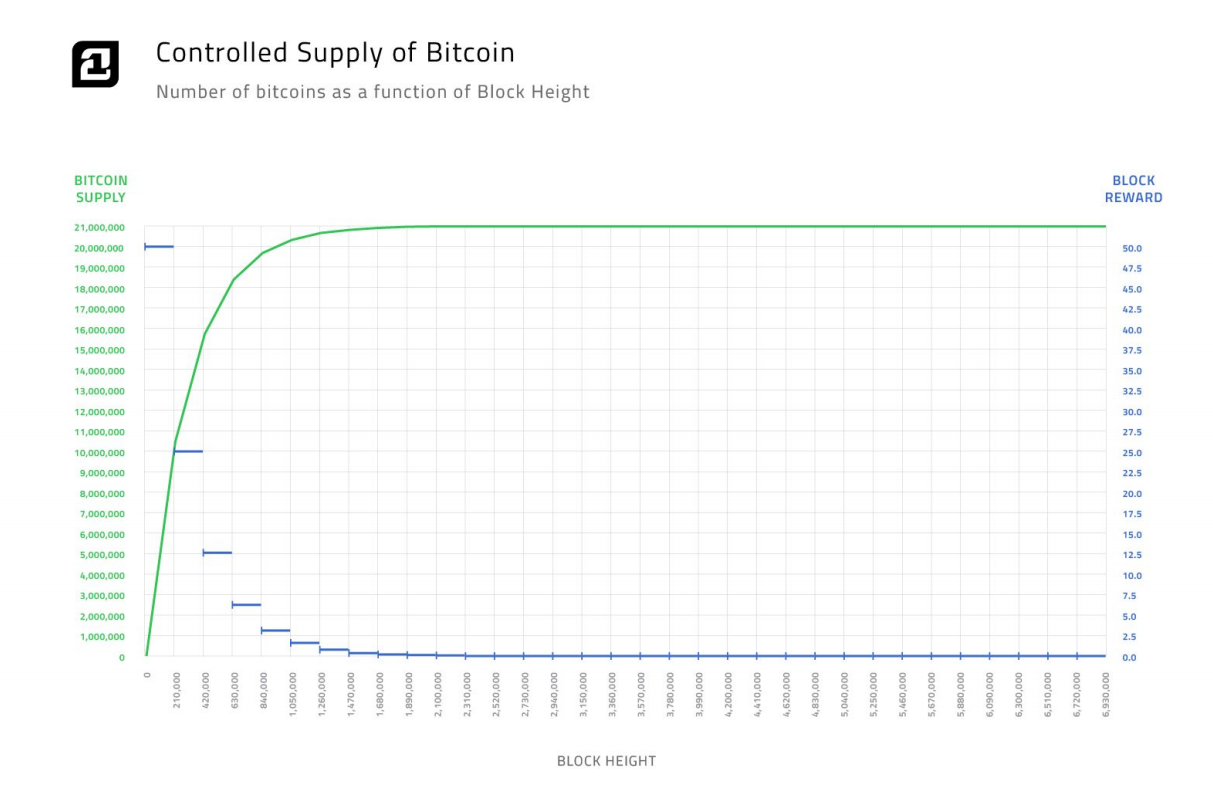
\includegraphics[scale=0.4]{supply_cap} \\
    
    \section*{Transaction Fees}
    
    The creator of a transaction sets the transaction fee. This is done voluntarily, but is practically necessary since it provides miners incentive to include the transaction above other transactions with high transaction fees. In practice, a higher transaction fee leads to a faster confirmation time. Transaction fees are a source of extra income for miners on top of the block reward, and are increasingly important as block reward diminishes over time. When block reward inevitably becomes 0, transaction fees will become the primary source of revenue for miners. To calculate transaction fee, simply subtract the output from the input amounts for the transaction. The difference implicitly becomes the transaction fee. 
    
    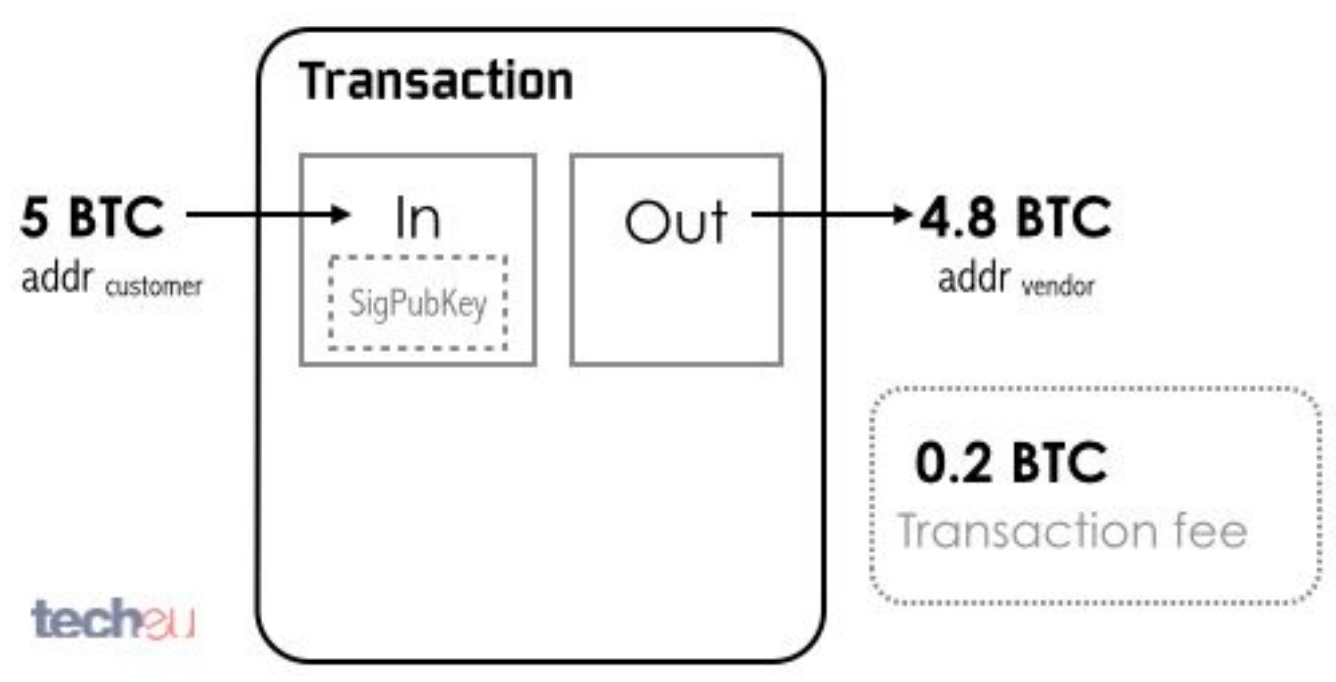
\includegraphics[scale=0.2]{transaction_fee} \\
    
    In the figure above, the input is 5 BTC and the output is 4.8 BTC. The creator of this bitcoin transaction has included an implicit transaction fee of 0.2 BTC that is to be collected by the miner who includes this transaction in the block that is confirmed by the rest of the network.

    \section*{Hardware Cost}
    
    In the beginning, most Bitcoin mining was done on CPUs. As the block difficulty increased however, mining efforts have shifted quite dramatically first to GPUs, then to FPGAs, and finally ASICs. CPU mining was accessible to anyone who wanted to try out the Bitcoin core software. Keep in mind that hardware costs are fixed, unlike everything else we have mentioned. 
    
    As commonly used CPUs began to get too slow for the block difficulty, GPU mining began to gain popularity. GPUs are an order of magnitude faster than CPUs in terms of hash power. However, this implies a larger consumption of energy and higher production of heat. GPU mining was most common around 5 years ago (2012), but as of now is not a viable solution for mining Bitcoin. (GPU mining is viable for Zcash on the other hand.) There were two main disadvantages to GPU mining:
    
    \begin{enumerate}
        \item GPUs have many components (like floating point units) that are not applicable to Bitcoin mining.
        \item GPUs are not meant to be run in ``farms'' side by side.
    \end{enumerate}
    
    The disadvantages of GPU mining made it clear that there needed to be a switch to mining specific hardware.
    
    \textbf{FPGAs (Field Programmable Gate Arrays)} were the result of early efforts to develop Bitcoin-specific hardware without losing all hardware customizability. It was essentially a trade-off between dedicated, specialized hardware to run only SHA-256, and more general purpose hardware. The reason that FPGAs seemed like such a compromise in hardware composition is because of lingering mistrust in the Bitcoin software. If Bitcoin failed, SHA-256 specific hardware would be worthless, but general purpose hardware would still be useful. However, if Bitcoin thrives, specialized hardware for churning out SHA-256 calculations would generate higher profit than generalized hardware.
    
    As Bitcoin continued to gain popularity, general purpose hardware was dropped altogether to create the first \textbf{ASICs (Application-Specific Integrated Circuits)}. ASICs do nothing but SHA-256, but does it better than any other hardware in the market. There are a huge variety of ASICs currently in the market, each with various tradeoffs. One obvious tradeoff is between base cost and electricity usage; this depends on how often the ASIC is to be run. Another is device size and hashrate; larger devices take up more space and user more electricity, but have a higher overall hashrate. Also, manufacturing ASICs takes large upfront capital, which induces centralization --- a tradeoff with Bitcoin's core decentralized philosophy. Currently, the most effective ASIC is the Antminer 29, which can output 14 TH/s, for the steep price of 3000 USD.
    
    \section*{Operating Costs}
    
    When considering the cost to operate Bitcoin mining equipment, it is useful to categorize cost into three primary categories. \textbf{Embodied energy} is the energy used to produce mining hardware. \textbf{Electricity} is used to power the hardware, and energy for \textbf{cooling} is required to maintain hardware health. All energy is converted to heat, which generally dissipates in the air and is wasted. However, there are initiatives to recapture heat generated from operating mining hardware. The ``data furnace'' is an idea that involves using mining hardware as a heater. An average household could mine bitcoin during the winter, heating up their home with left over thermal energy from mining equipment, and earning a little profit on the side too. 
    
    \section*{ASIC-Resistance --- Pros and Cons}
    
    \textbf{ASIC-resistance} is the idea that mining should not be sped up with specialized hardware --- that there should be no significant speedup by implementing a mining algorithm in an ASIC, as compared a CPU based implementation. ASICs are currently the only viable option when it comes to mining bitcoin in the present day, since they are designed with the sole purpose of calculating SHA-256. Thus, ASICs dominate the Bitcoin network, and suppress regular people. If Bitcoin were to be ASIC-resistant, there would be an increase in democracy and decrease in centralization, as ASIC farms would have less power over the average CPU miner.
    
    However, there is also a strong case against ASIC-resistance. ASICs can only solve the Bitcoin hash puzzle, nothing more. If there is a crash in exchange rate, ASICS would be rendered to useless electricity-gobbling hardware. (Attackers could rent general computing resources, however, resulting in no wasted investment.) Investment into expensive ASIC hardware becomes worthless without a puzzle to solve, so this discourages attacks on the Bitcoin network. The existence of ASICs then ensure the network's security to a certain extent.
    
    \section*{ASIC-Resistance --- Memory-Hard Puzzle}
    
    Movements to make Bitcoin ASIC-resistant have stirred debate on the usage of \textbf{memory-hard puzzles}, which require large amounts of memory, rather than computational power, to solve. These puzzles would be \textbf{memory-bound}, meaning that memory bottlenecks computation time. Memory-hard puzzles would viably deter ASICs and effectively make Bitcoin ASIC-resistant. ASICs are optimized to compute a specific algorithm, while regular CPUs are not, and since optimization of this algorithm (SHA-2556) is not the limiting agent, ASICs would not give certain miners more power over others. Memory is the limiting agent, not computational optimization. Memory performance increases much slower than computational power. The cost of solving a puzzle also decreases much slower. These considerations have all made the debate of ASIC-resistance an important topic among users in the Bitcoin network.
    
    \section*{Scrypt}
    
    \textbf{Scrypt} (pronounced ``ess crypt'') is an algorithm used by Litecoin and Dogecoin for computing proof-of-work hashes. Scrypt was designed to be used for hashing passwords and hard to brute-force. To do so, scrypt requires a large amount of memory compared to other algorithms, making the size and cost of potential specialized hardware much more expensive than those for other algorithms. 
    
    Scrypt has two main steps. A user must first fill a buffer with interdependent (pseudorandom) data. Then, the user accesses the memory buffer in a pseudorandom way until a correct hash is found. The drawback is that scrypt requires equal amount of memory to verify. Scrypt ASICs have also been developed, so in practice, scrypt is far from being ASIC-resistant.
    
    \section*{ASIC-Resistance --- Other Approaches}
    
    Memory-hard algorithms such as scrypt do not provide real-world ASIC-resistance. Initiatives such as using technologies such as \textbf{x11} and \textbf{x13} hash function chaining have been proposed and implemented. The cryptocurrency DASH currently uses x11, and chains together 11 different hash functions. Designing ASICs for x11 and x13 systems are significantly harder than designing ASICs for Bitcoin, but is technically not impossible.
    
    There is also the idea of periodically switching a mining puzzle. For example, a cryptocurrency system could go from SHA-1 to SHA-3 to Scrypt every 6 months. However, this solution is easy to work around, if one were to know the rotation of such mining puzzles. This solution has also not been implemented yet. In short, ASIC-resistance seems to be an impossible goal. As Mike Hearn, Bitcoin Core developer has famously stated: ''There's really no such thing as an ASIC-resistant algorithm.''
    
    \section*{Proof-of-Useful-Work}
    
    Instead of having the world's most powerful network of computers incrementing and recalculating what is essentially just one math problem, why not have this massive collective of computational power do some useful work? This is the main motivation of \textbf{proof-of-useful-work}, which aims to repurpose the computational power of a Proof-of-work cryptocurrency network to solve important problems. Historically, long-term public research projects have produced great findings, and Proof-of-useful-work encourages this by attempting to repurpose mining compute power to aid:
    
    \begin{itemize}
        \item Searching for large primes --- Great Internet Mersenne Prime Search, which found the ``largest prime number'' to date ($2^{57885161} - 1$) twelve straight times.
        \item Finding aliens --- Seti@home, which is the largest project to date, with over 5 million participants.
        \item Simulating proteins at the atomic level --- Folding@home, which has the greatest computing capacity of any volunteer computing project, and has produced more than 118 scientific papers. 
        \item Securing cryptography --- distributed.net, which was the first successful public brute-force of a 61-bit cryptographic key.
        \item Generating predictive climate models 
        \item Producing solar power (Solarcoin distributes coin to those who can produce solar power.)
    \end{itemize}
    
    As good as Proof-of-useful-work sounds, there are some design restrictions that make it less than ideal in consideration of cryptocurrencies and blockchain. Many distributed computing problems are unsuitablle for proof-of-work. There is always a fixed amount of data that users have access to. For example, contributers to SETI@Home could run out of raw radio telescope data, leaving no problem to solve. Distributed computing problems are missing an inexhaustible puzzle space. Secondly, potential solutions to these computing problems are not equally likely, so there is a lack of equiprobably solution space. Thirdly, we must not rely on a central entity to delegate tasks, otherwise fail to reach the requirement of decentralized and algorithmically generating problems. Thuss, Proof-of-useful-work is mostly unviable.
    
    \section*{Proof-of-Storage --- Permacoin}
    
    Instead of distributing work across a network, one idea involves distributing large files. In \textbf{Proof-of-storage}, specifically the Permacoin implementation, a large public file in need of replication is split. An example of such a file would be experimental data from the Large Hadron Collider, which has several hundred petabytes of data. Such a file would be stored in blocks, in a Merkle tree upon which the network agrees. Each miner then stores a subset of these blocks, $T$, based off their public key. They then continuously hash consensus information with a nonce to pick blocks in their stored subset. The goal is to find a nonce such that its hash with all block headers is less than some target. Each server can query a given index, which returns a block header for the public data. One drawback to Proof-of-storage is that it is hard to find such a large a file to subsection to the network's nodes. If such a file is found, it would be difficult to change the block difficulty, or to modify the file.
    
    \section*{Merge Mining}
    
    Consider the potential vulnerabilities of a new altcoin in the current market. Lack of hashpower in the altcoin's network correlates to a lack of security. It is easy for an individual to amass enough hash power to attack the network, since the network is small. Mining however is exclusive by default. What is the incentive to mine and attack an altcoin if you can make profit on the Bitcoin blockchain? Despite this lack of coin/cash incentive, historically, there have been cases of ``altcoin infanticide.'' Altcoins with their minimally connected networks are vulnerable to attacks from larger coins (Bitcoin). An individual Bitcoin miner or pool may have much more hash power than that of the entire altcoin. In 2012, Eligius mining pool attacked CoiledCoin, reversing multiple days' worth of transactions.
    
    The solution to the problem of altcoins being too weak is to implement \textbf{merge mining}. Merge mining involves creating blocks with transactions from both Bitcoin and an altcoin. Altcoins could be designed however desirable; the problem would be how to incentivise miners to include altcoin transactions in Bitcoin. Solving this requires including a Merkle root of altcoin transactions in Bitcoin's coinbase parameter. Bitcoin miners could then reap both Bitcoin and altcoin rewards. This would result in no additional cost, and no profit loss at all. \\
    
     
   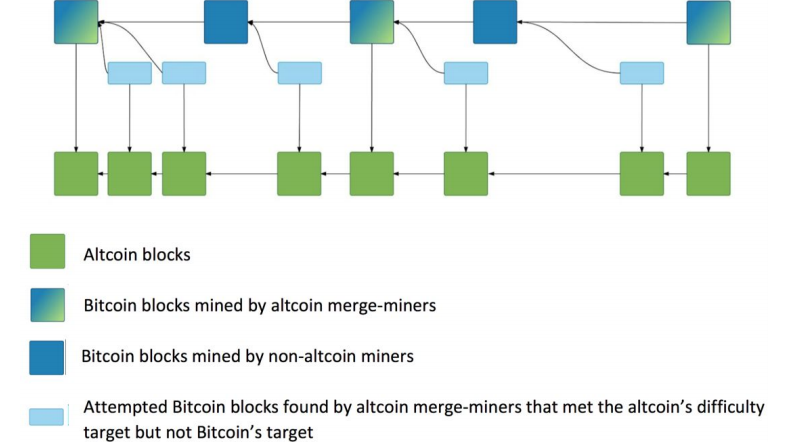
\includegraphics[scale=0.5]{merge} \\
   
    
    
    % BEGIN KEY TERMS
    \newpage
    \thispagestyle{firstpage}
    \vspace*{2\baselineskip}
    \section*{Key Terms}
    \noindent A collection of terms mentioned in the note which may or may not have been described. Look to external sources for deeper understanding of any non-crypto/blockchain terms.
    \begin{enumerate}
        % edit within here
        \item \textbf{VOCAB WORD} --- Definition. % format
    \end{enumerate}
    % END KEY TERMS
\end{document}